\documentclass[a4paper]{article}

%%%%%%%% CREATE DOCUMENT STRUCTURE %%%%%%%%
%% Language and font encodings
\usepackage[english]{babel}
\usepackage[utf8x]{inputenc}
\usepackage[T1]{fontenc}
%\usepackage{subfig}

%% Sets page size and margins
\usepackage[a4paper,top=3cm,bottom=2cm,left=2cm,right=2cm,marginparwidth=1.75cm]{geometry}

%% Useful packages
\usepackage{amsmath}
\usepackage{graphicx}
\usepackage[colorinlistoftodos]{todonotes}
\usepackage[colorlinks=true, allcolors=blue]{hyperref}
%\usepackage{caption}
\usepackage[justification=centering]{caption}
\usepackage{subcaption}
\usepackage{sectsty}
\usepackage{float}
\usepackage{titling} 
\usepackage{blindtext}
\usepackage[square,sort,comma,numbers]{natbib}
\usepackage[colorinlistoftodos]{todonotes}
\usepackage{xcolor}
\usepackage{fancyhdr}
\usepackage{lipsum}

%% definitions 
\definecolor{darkgreen}{rgb}{0.0, 0.4, 0.0}

%% Define your personal info here %%%%%%%%%%%%%%%%%%%%%%%
\newcommand\TPid{2}
\newcommand\TPname{HVS Perception and Colors}
\newcommand\Firstname{Joao Filipe}
\newcommand\Familyname{Costa da Quinta}
\newcommand\Email{Joao.Costa@etu.unige.ch}
%%%%%%%%%%%%%%%%%%%%%%%%%%%%%%%%%%%%%%%%%%%%%%%%%%%%%%%

%%%%%%% Page header %%%%%%
\pagestyle{fancy}
\fancyhf{}
\rhead{TP \TPid: \TPname}
\lhead{\Firstname \; \Familyname}
\rfoot{Page \thepage}


%%%%%%%% DOCUMENT %%%%%%%%
\begin{document}

%%%% Title Page
\begin{titlepage}

\newcommand{\HRule}{\rule{\linewidth}{0.5mm}} 							% horizontal line and its thickness
\newcommand\tab[1][1cm]{\hspace*{#1}}
\center 
 
% University
\textsc{\LARGE Université de Genève}\\[1cm]

% Document info
\textsc{\Large Imagerie Numérique}\\[0.2cm]
\textsc{\large 13X004}\\[1cm] 										% Course Code
\HRule \\[0.8cm]
{ \huge \bfseries TP \TPid : \TPname}\\[0.7cm]								% Assignment
\HRule \\[2cm]
\large
\emph{Author:} \Firstname \; \Familyname\\[0.5cm]		
\emph{E-mail:} {\color{blue}\Email}\\[7cm]		
% Author info
% Author info
{\large \today}\\[2cm]

\includegraphics[width=0.4\textwidth]{images/unige_csd.png}\\[1cm] 	% University logo
\vfill 
\end{titlepage}


% ============================================
% ----------------------------------
\section*{Exercise 1}
\begin{itemize}
\item[(a)] There are two main components in the HVS, first of there is ofcourse the sensory organ (eye) that senses light, and then there is the brain that processes the information, this is information is transmited by the optic nerve.
\item[(b)] The light that we perceive is in the range is from 350 nm to 780 nm, this light is detected by the retina, that is equiped with two types of cells that detect an respond to light, rods and cones, rods are responsible for the achromatic light (dark environment) and we have 100 million rods, the cones however are responsible for the well lighted environment, but we only have 6.5 million, much fewer, they are also very concentrated in one place within the eye.
\end{itemize}

% ----------------------------------
\section*{Exercise 2}
\begin{center}
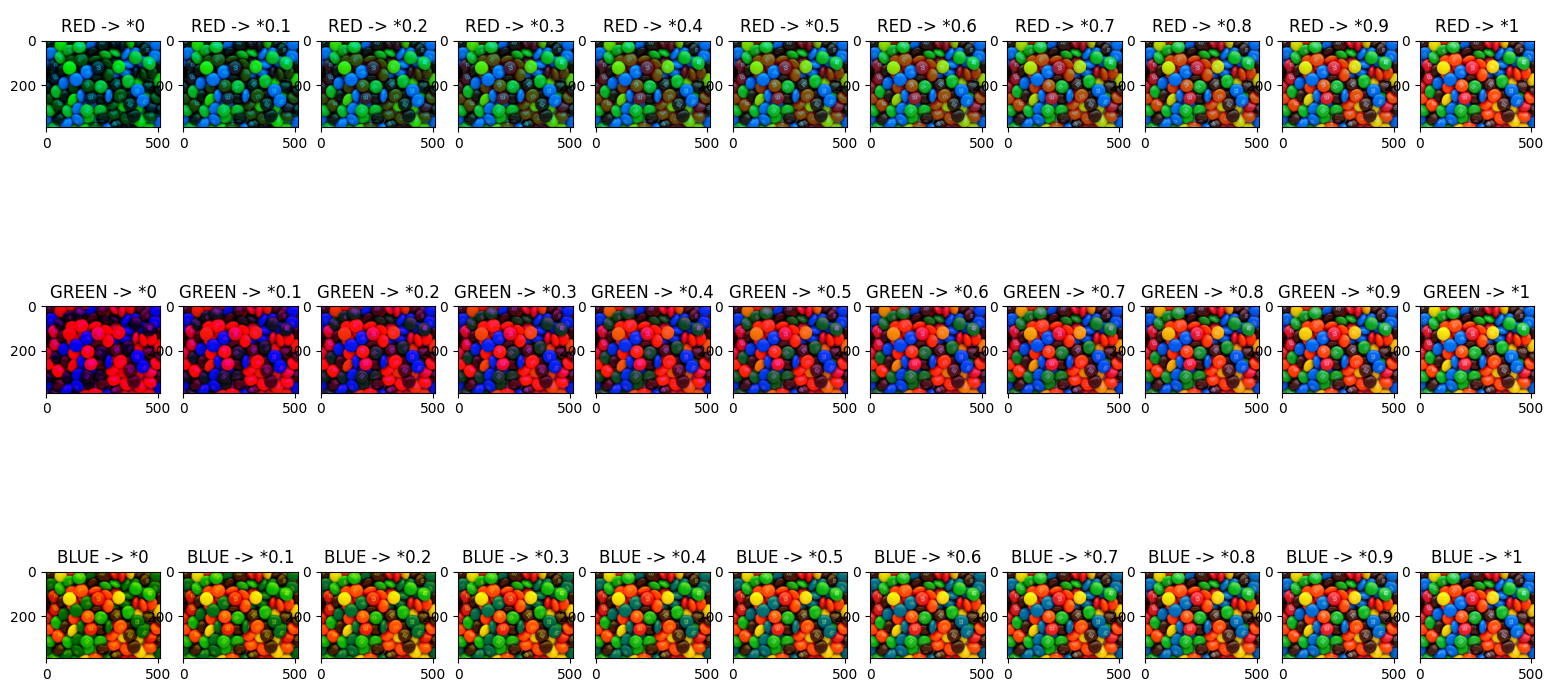
\includegraphics[width=1\textwidth]{images/exercice_2.PNG}\\[1cm] 
\end{center}
The results are as expected, in last TP we kept the red accent color turning green and blue down, here we do the opposite, we scale the red color from 0$\%$ to 100$\%$, we clearly see the lack of the scaled down color at 0$\%$, and we can withness it gradually apearing more and more as we get closer to 100$\%$.
% ----------------------------------
\section*{Exercise 3}
\begin{itemize}
\item[(a)] The YIQ is the color space used by NTSC color system in the USA, Y represents the luma component, I the orange-blue range of colors and Q the purple-green.
\item[(b)]
\begin{center}
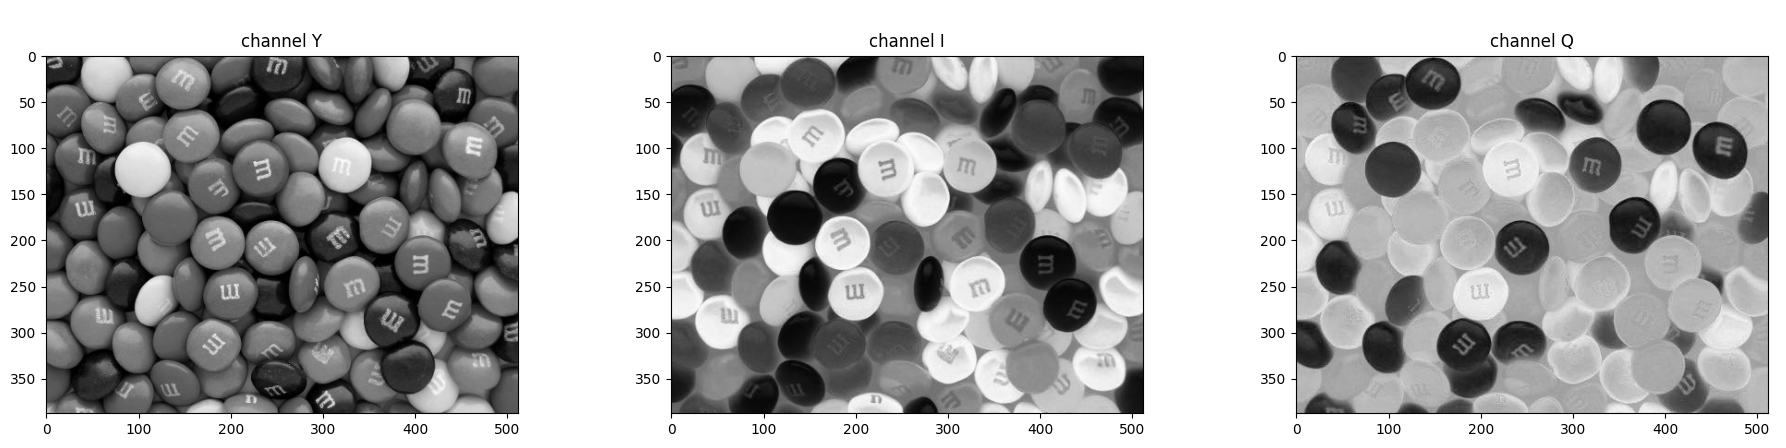
\includegraphics[width=1\textwidth]{images/exercice_3_b.PNG}\\[1cm] 
\end{center}
\item[(c)]
\begin{center}
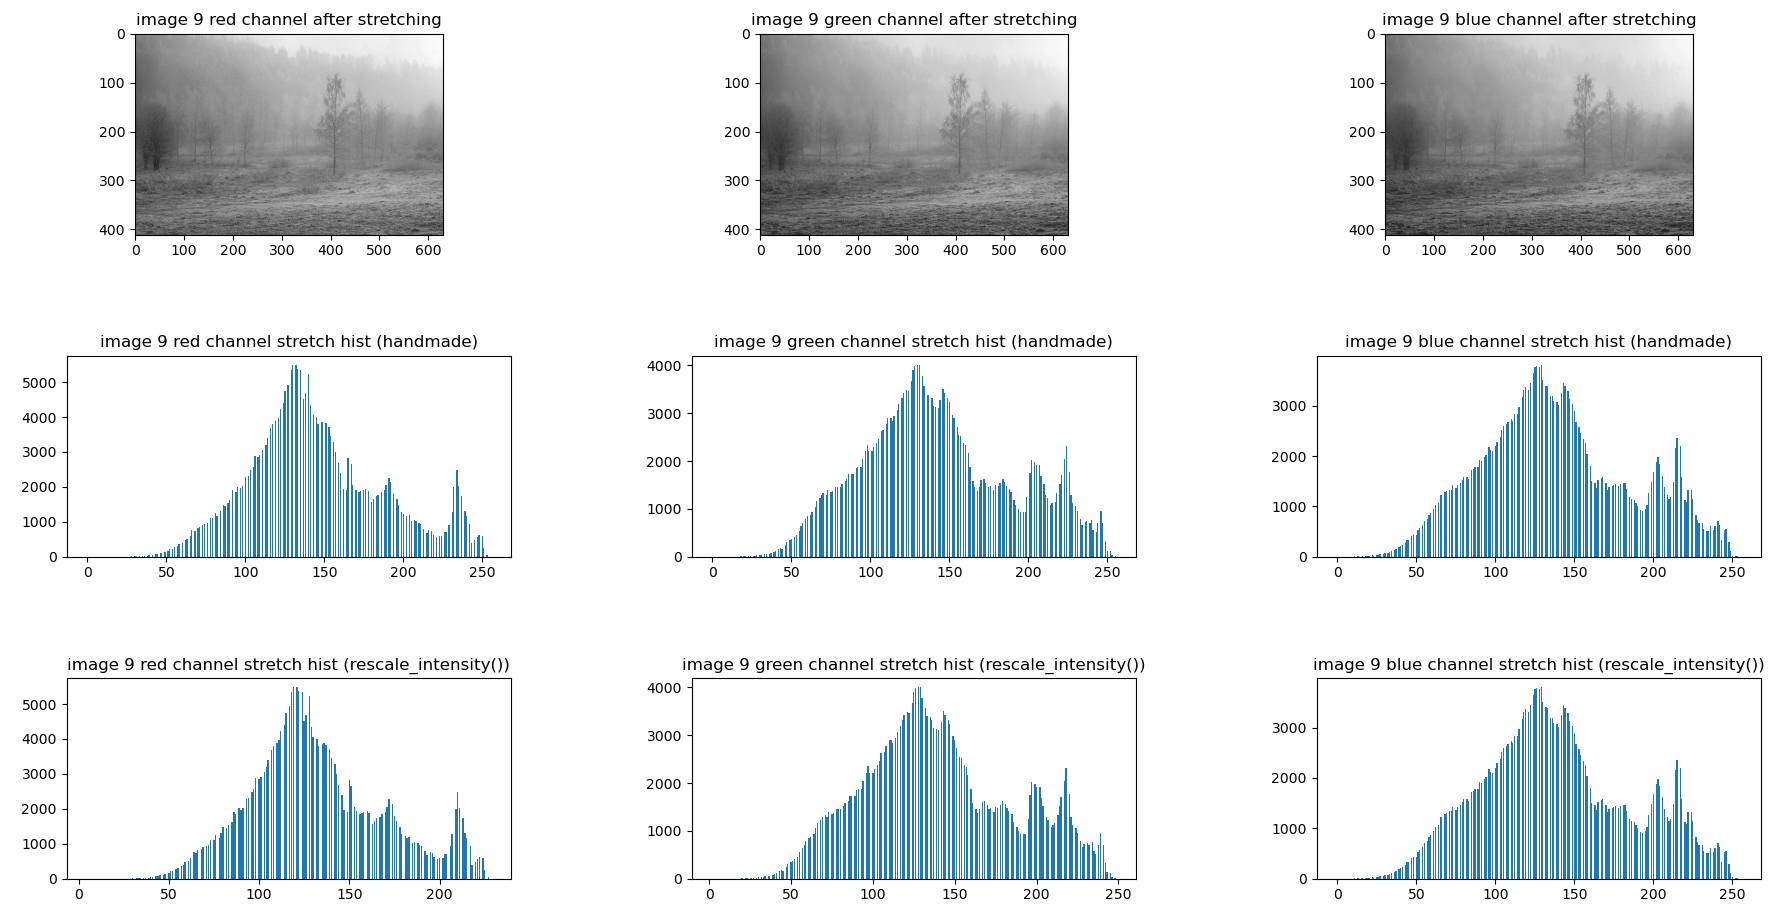
\includegraphics[width=1\textwidth]{images/exercice_3_c.PNG}\\[1cm] 
\end{center}
\item[(d)] The mse is = 14490.1831, this is very interesting, despite this big change in mse, they look visually the same. 
\end{itemize}
% ----------------------------------
\section*{Exercise 4}
\begin{itemize}
\item[(a)] The Y'UV is the color space used by PAL color analog TV system , and YCbCr is the digital equivalent, Y' represents the luma component, U represents the blue difference component and V the red difference component.
\item[(b)]
\begin{center}
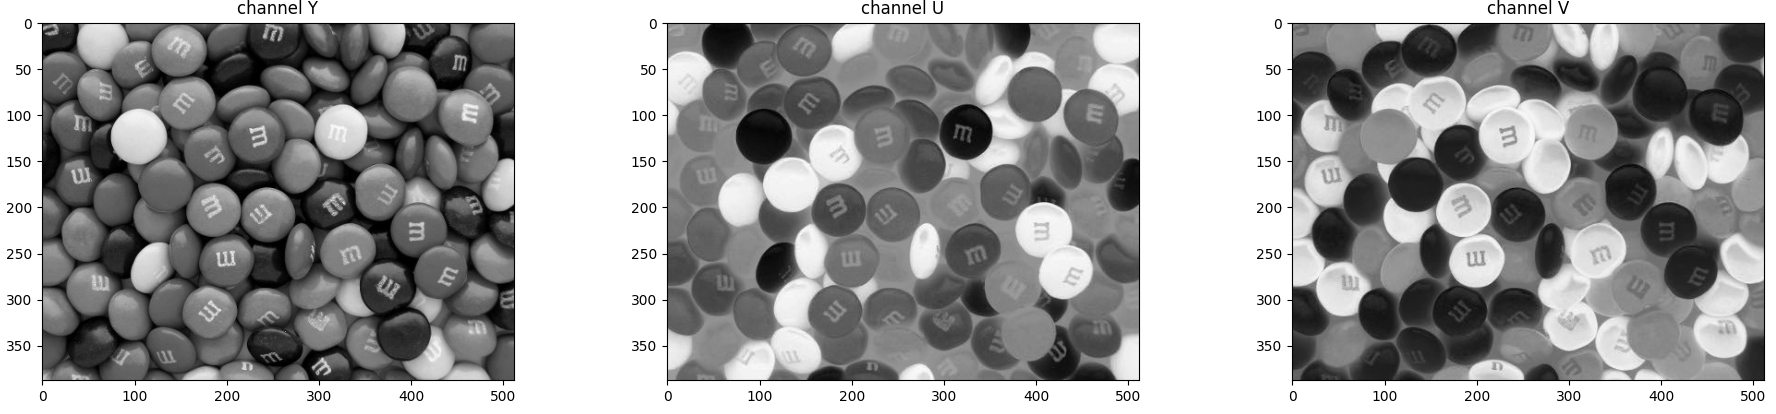
\includegraphics[width=1\textwidth]{images/exercice_4_b.PNG}\\[1cm] 
\end{center}
\item[(c)]
\begin{center}
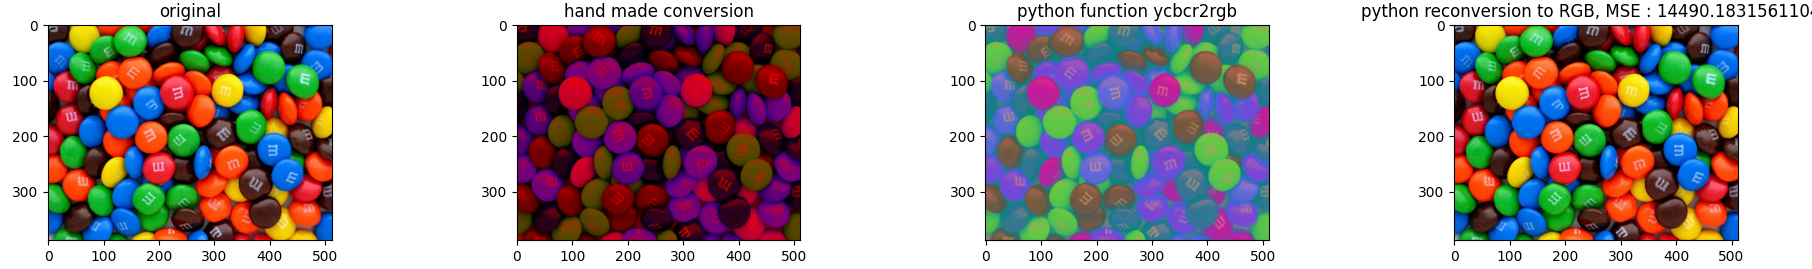
\includegraphics[width=1\textwidth]{images/exercice_4_c.PNG}\\[1cm] 
\end{center}
\item[(d)] The mse is = 14490.1831, this is very interesting, despite this big change in mse, they look visually the same. 
\end{itemize}
% ----------------------------------
\section*{Exercise 5}
\begin{itemize}
\item[(a)] The CMY system is the complementary system of the RGB color scheme, we already saw it in this TP in exercice 2. Cyan is the mixture of Green and Blue, which is the same, as subtracting Red from White, which is litterally what we did in Exercice 2, we gradually substract Red, leaving Green and Blue, that is why the mnms are all of very close the the Cyan color. Using the same logic, Magenta is created from substracting Green from White, and finally, Yellow is is created from substracting Blue from White.
\item[(b)]
\begin{center}
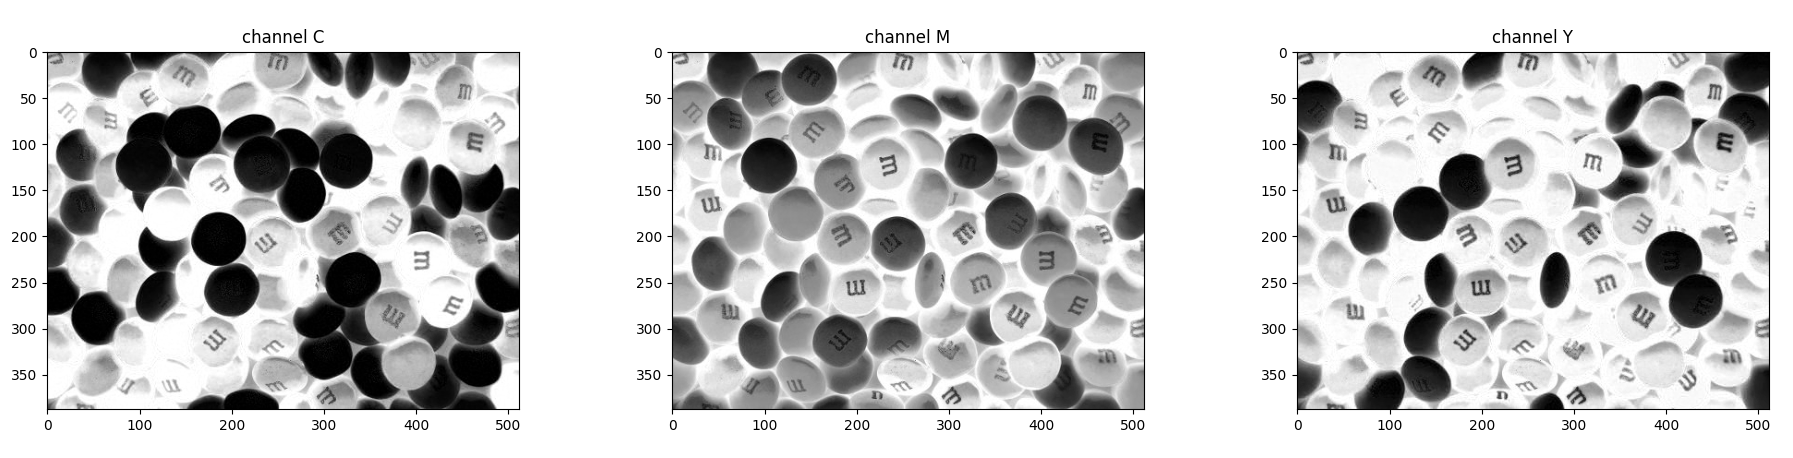
\includegraphics[width=1\textwidth]{images/exercice_5_b.PNG}\\[1cm] 
\end{center}
\item[(c)]
\begin{center}
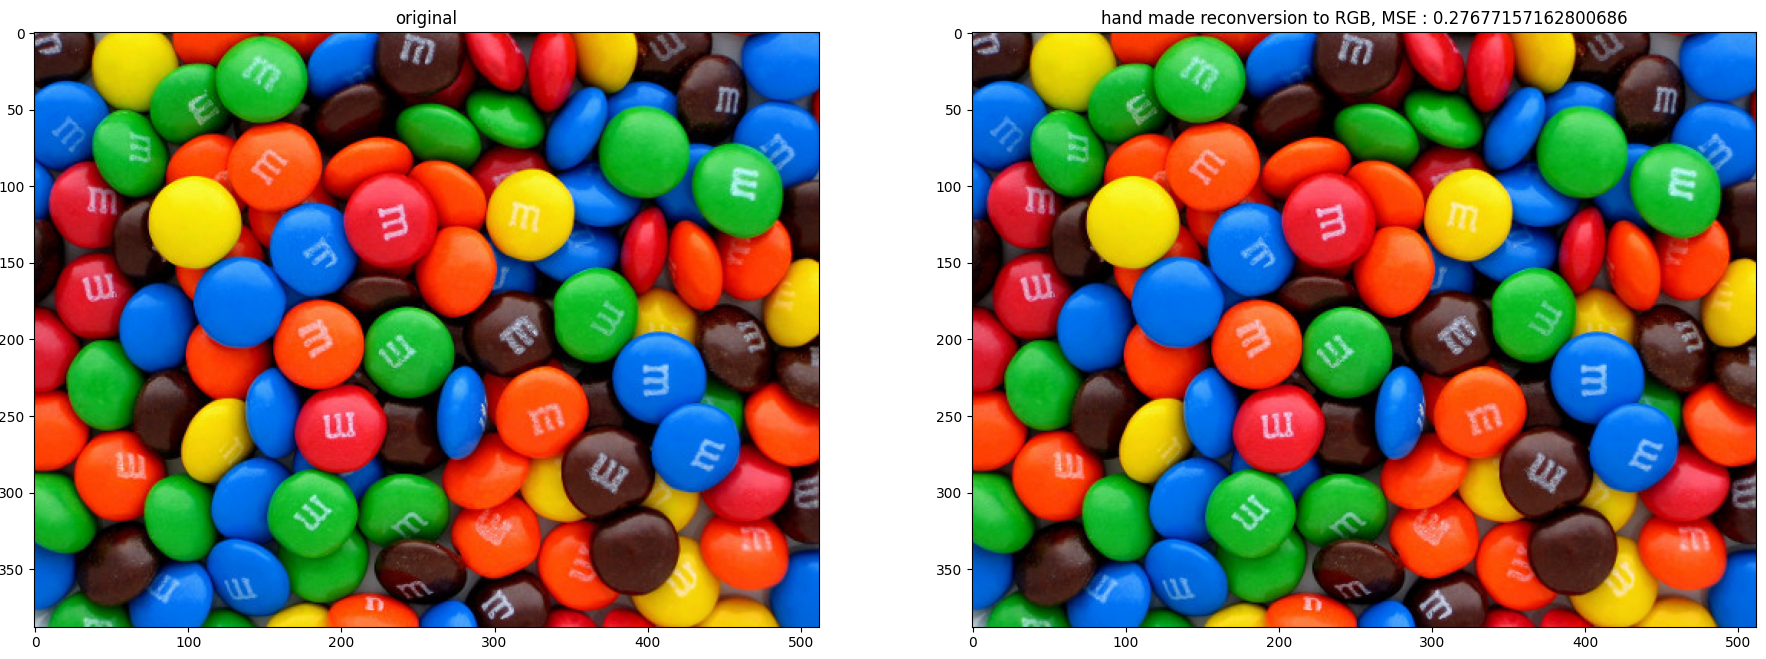
\includegraphics[width=1\textwidth]{images/exercice_5_c.PNG}\\[1cm] 
\end{center}
\item[(d)] The mse is = 0.27677, not much information was changed after all the computations.
\end{itemize}

% ----------------------------------
\section*{Exercise 6}
\begin{itemize}
\item[(a)] With the CMY system we have 3 different channels, as we can see in the images above, however, in the CMYK we have 4 different colors, K represents the color Black, K is computed as follows K = min(C,M,Y) and then we recompute C,M,Y as C = C - K (same for M and Y), this is done so we waste less ink, as we can replace a bit of Cyan a bit of Magenta and a bit of Yellow by Black, so we end up with 4 color channels. This is used today for printers, as it is less expensive to print CMYK than CMY.
\item[(b)]
\begin{center}
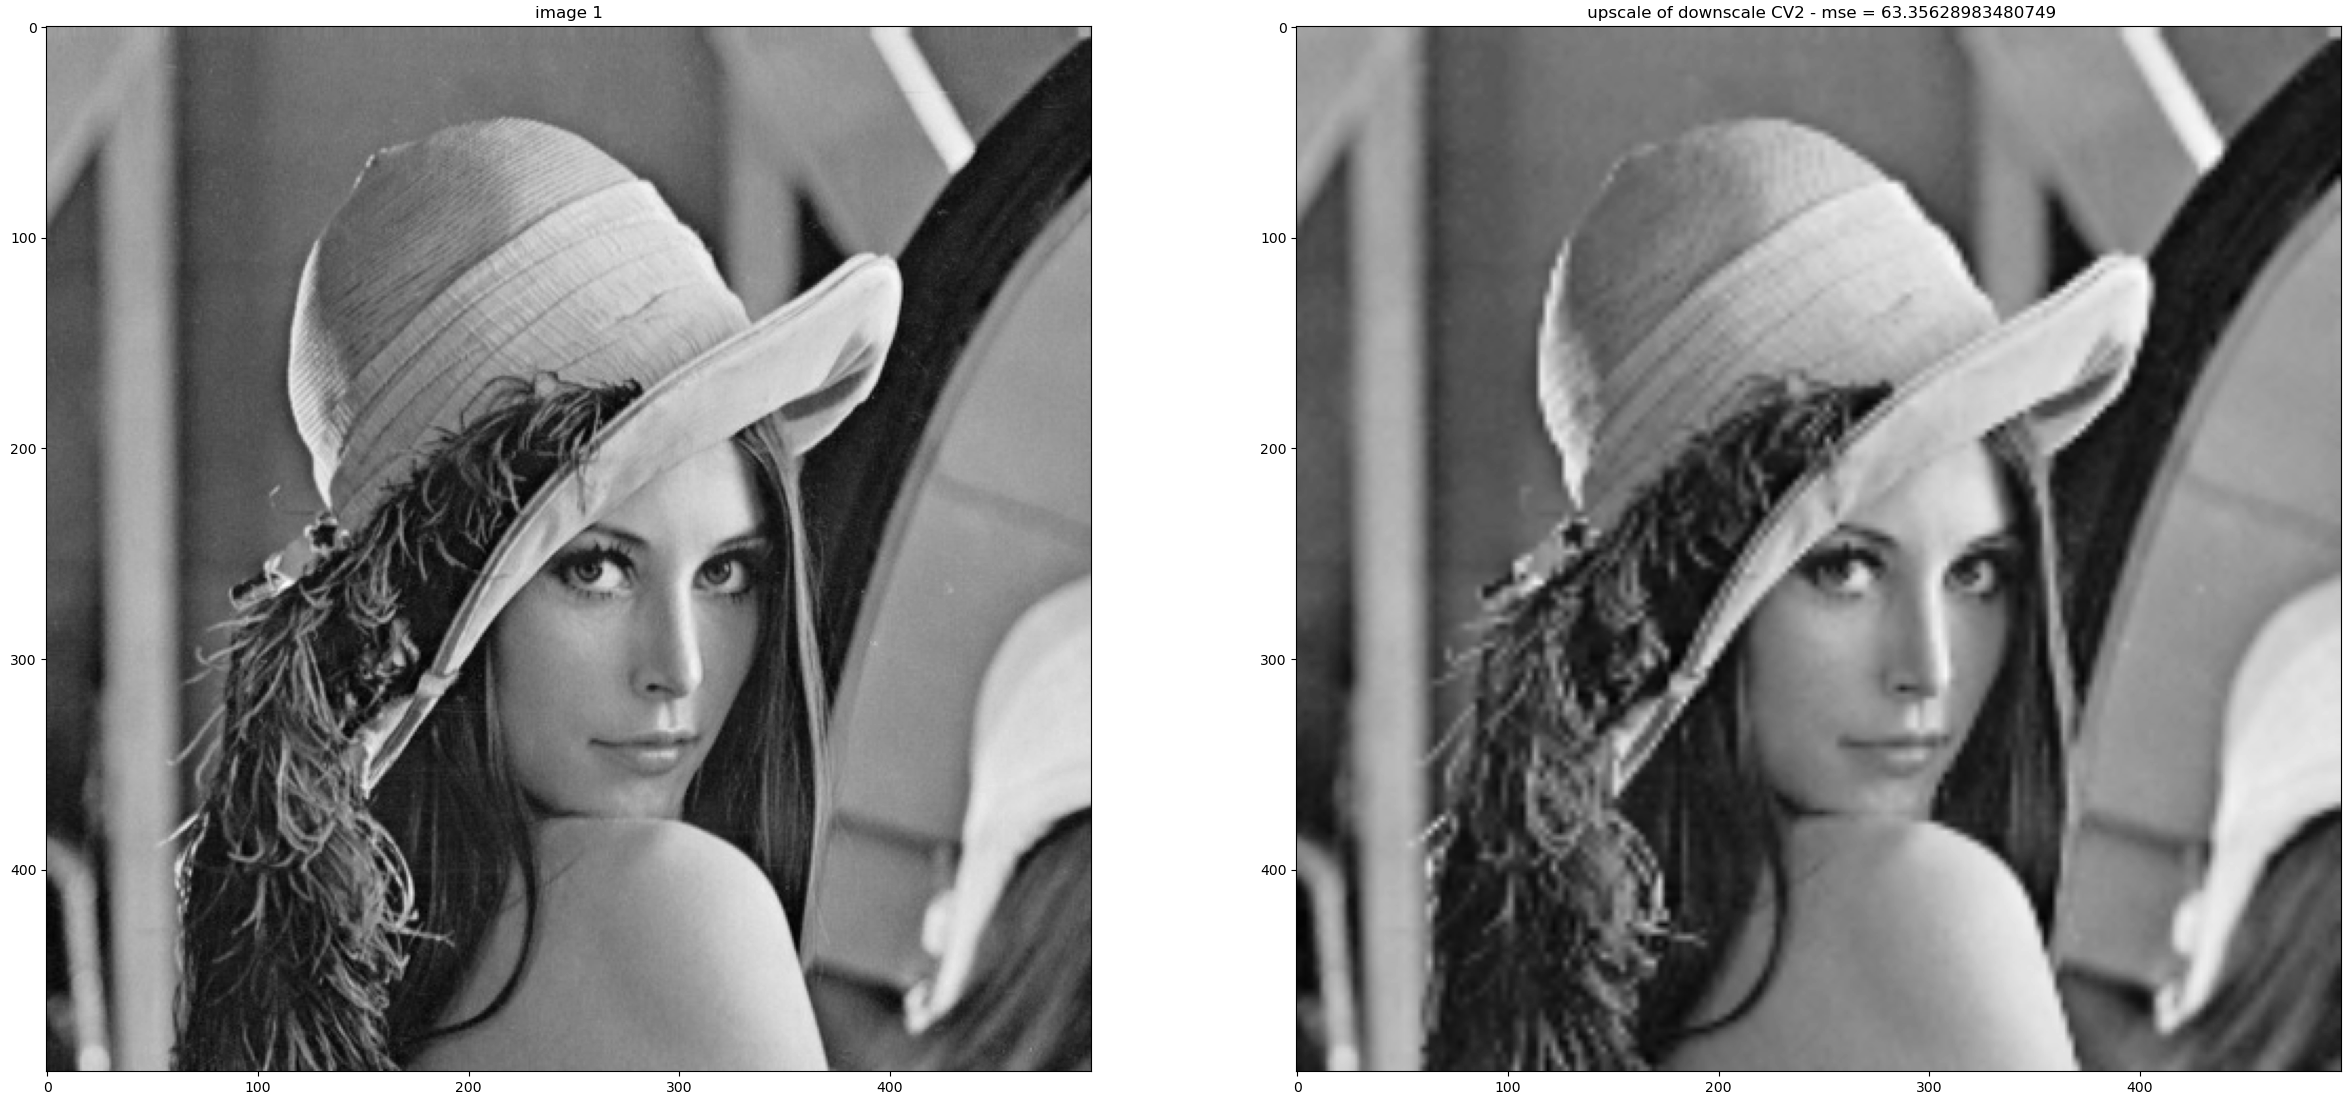
\includegraphics[width=1\textwidth]{images/exercice_6_b.PNG}\\[1cm] 
\end{center}
\item[(c)]
\begin{center}
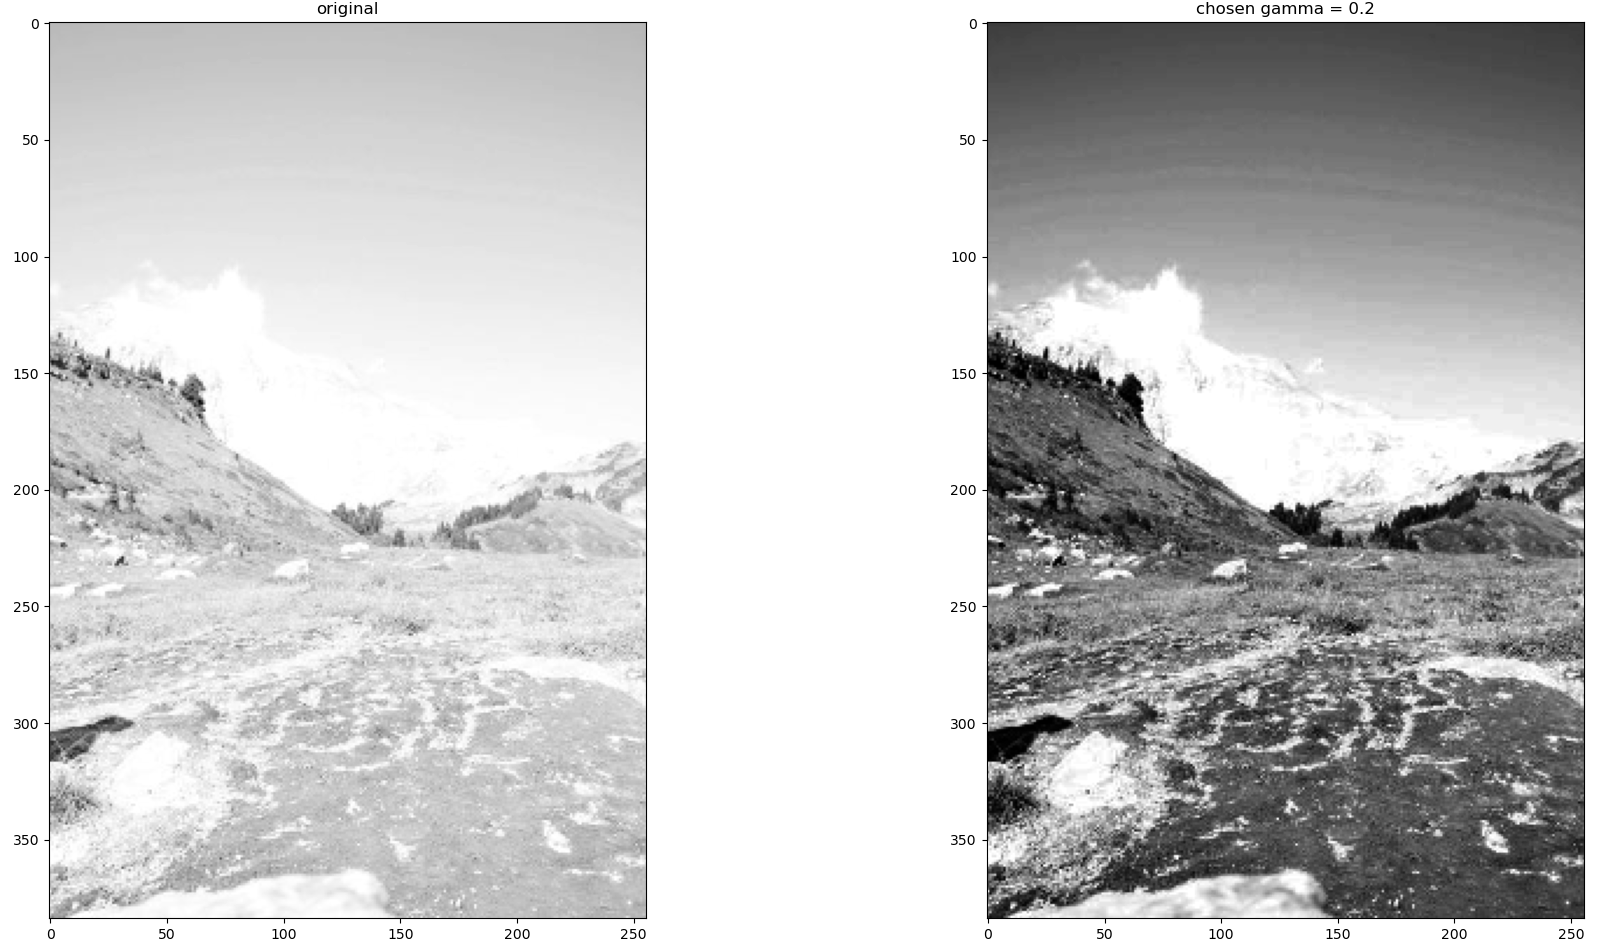
\includegraphics[width=1\textwidth]{images/exercice_6_c.PNG}\\[1cm] 
\end{center}
\item[(d)] The mse is = 0.27677, not much information was changed after all the computations.
\end{itemize}

% ----------------------------------
\section*{Exercise 7}
\begin{itemize}
\item[(a)]
\begin{itemize}
\item[Emmetropia] This condition is when a far away object is perceived by the human eye in sharp focus and the lens is relaxed, meaning the eyes "normal" focus is on a distance, and to focus somewhere else the individual does it consciously. No corrective lenses are required, however surgery is possible.
\item[Myopia] Is an eye disorder where far away objects are perceived as blurry, this is due to the fact that the light focuses in front of the retina instead of on the retina, to correct this probelm an idividual may where corrective lenses that bend the light entering the eye in such a way that the focused image is placed correctely on the retina, this condition can also be corrected via surgery.
\item[Hypermetropia] As oppose to Myopia where the light focuses in front of the retina, in hypermetropia the light focuses behind the retina, the treatment follows the same idea as the treatment for Myopia, corrective lenses so that the image is focused on the retina, or surgeries for a more permanent correction.
\item[astigmatism] This condition is due to the fact that the eye does not focus light evenly on the retina, this results in blurred vision at any distance, the same kinds of treatment are availeable, however eyeglasses are the safest aproach.
\end{itemize}
\begin{center}
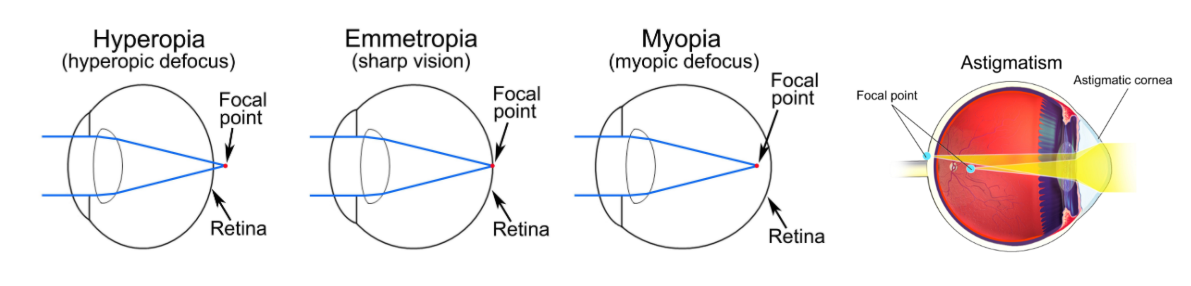
\includegraphics[width=1\textwidth]{images/exercice_7_a.PNG}\\[1cm] 
\end{center}
\item[(b)] Both the eye and a camera are equiped with a lens, in a camera, to focus the image we change the distance between the lens and the image plane, however, in the Human brain we can't simply move sinse the distance between the center of the lens and the retina is fixed, so to focus we change the focal distance by varying the lens.
\end{itemize}

% ----------------------------------
\end{document}